\documentclass[a4paper,12pt]{report}
\setcounter{tocdepth}{3}

\usepackage{alltt, fancyvrb, url}
\usepackage{graphicx}
\usepackage[utf8]{inputenc}
\usepackage{float}
\usepackage{hyperref}

% Questo commentalo se vuoi scrivere in inglese.
% \usepackage[italian]{babel}

\usepackage[italian]{cleveref}

\title{Relazione Progetto OOP\\``Dimension Holiday''}

\author{Lorenzo Prati, Elvis Perlika\\ Emanuele Dajko, Alessandra Versari}
\date{\today}


\begin{document}

\maketitle

\tableofcontents

\chapter{Analisi}

\section{Requisiti}

Il gruppo si pone l'obbiettivo di realizzare un videogioco roguelike \textit{Dimension Holiday} vagamente ispirato a giochi famosi come \textit{Hades} oppure \textit{The Binding of Isaac}. Il giocatore controllera' un personaggio 
esplorare un dungeon composto di diverse stanze e affrontare un boss per vincere il gioco.

\subsection*{Elementi funzionali}

\begin{itemize}
	\item Per attraversare tutto il dungeon il giocatore dovrà passare da stanza in stanza,
	eliminando tutti i nemici presenti. Per farlo potrà usare la spada, lanciare
	proiettili o utilizzare una magia di fuoco. Giocatore e nemici hanno delle vite (espresse in cuori) e se il giocatore perde tutti i cuori e' \textit{Game over} e si deve ricominciare da capo
	\item Una volta che il giocatore avrà ucciso tutti i nemici della stanza corrente un portale (\textit{Gate}) che e' presente nella stanza potra' essere attraversato per passare alla stanza successiva
	\item Dopo un certo numero di stanze, comparirà una stanza shop
	dove sarà possibile effettuare acquisti usando le monete creando una piccola progressione
	\item Il gioco si conclude quando il giocatore sconfigge un nemico speciale chiamato \textit{Boss}
	
\end{itemize}

\subsection*{Elementi non funzionali}

\begin{itemize}
	\item Ci si pone l'obbiettivo di creare un'architettura del software modulare ed espandibile ad aggiunte future, come l'aggiunta di nuovi nemici, mappe e oggetti.
\end{itemize}


\section{Analisi e modello del dominio}
Il giocatore potra' muoversi nelle 4 direzioni su, sinsitra, giu', destra tramite i tasti, rispettivamente, W, A, S, D ed effettuare due tipi di attacchi piu' un'abilita' speciale:
\begin{itemize}
	\item un attacco ravvicinato, usando la sua spada e tramite il tasto sinistro del mouse
	\item un attacco dalla distanza, usando un proiettile energetico e tramite il tasto destro del mouse
	\item un attacco caricato, tenendo premuto il tasto Z per 3 secondi e rilasciandolo per sparare una palla di fuoco che fara' piu' danno di un normale proiettile
\end{itemize}
Il gioco dovra' essere in grado di presentare al \texttt{giocatore} una serie di stanze dove affrontare dei \texttt{nemici}. Questi potranno avere diversi comportamenti e diverse tipologie di \texttt{attacco}. Il giocatore dovrà stare attento ad evitare gli attacchi dei nemici per non perdere cuori. I nemici possono attaccare sia dalla distanza con dei proiettili sia da vicino. Quando un'entita' esaurisce i cuori, essa deve essere rimossa dal \texttt{mondo} di gioco; inoltre alla rimozione di determinate entita' il gioco puo' reagire in diversi modi, ad esempio decretando il \textit{Game over} nel caso il player muoia, oppure la vittoria nel caso il boss venga sconfitto.
Saranno presenti degli \texttt{oggetti} raccoglibili (cuori, monete ecc.) che dovranno applicare degli effetti alle entita' con cui entrano in contatto, ad esempio l'incremento della vita oppure l'incremento della valuta posseduta dal giocatore. 
Lo shop sara' gestito \textit{in game}, nel senso che non comparirà un'interfaccia grafica che permettera' al giocatore di scegliere i potenziamenti, ma il giocatore dovra' interagire dinamicamente con degli oggetti presenti nella mappa per acquistarli.
Anche gli attacchi applicheranno degli effetti alle entita' con cui entrano in contatto, come ad esempio la perdita di cuori.
Il \texttt{mondo} di gioco  sara' composto di una serie di \texttt{stanze}. Tramite l'interazione con un oggetto portale, il giocatore sara' trasportato alla stanza successiva senza possibilità di tornare indietro. All'interno delle stanze sono presenti dei muri, che bloccano il passaggio al giocatore. Esistono tre tipi di stanze: normale, shop, boss. Nella stanza normale compariranno dei nemici e alcuni oggetti raccoglibili, in numero e tipo casuale; nella stanza shop invece compariranno gli oggetti rappresentanti i potenziamenti acquistabili, e nella stanza boss comparirà il nemico boss.

Una delle maggiori difficoltà consistera' nella creazione di un architettura che permetta la gestione sia di diversi tipi di nemici (zombie, shooter, boss ecc.), ognuno con un proprio comportamento, sia di diversi attacchi utilizzabili sia dal giocatore che dai nemici (proiettili, attacchi meele). Inoltre, si cerchera' di realizzare un sistema di combattimento \textit{action} e \textit{real-time} quanto piu' possibile fluido e responsivo e un'alternanza di mappe e generazione dei nemici in modo tale da far sembrare ogni partita diversa.

Dato il monte ore previsto, si rimanda al futuro una gestione accurata delle performance del gioco.


\begin{figure}[h]
	\centering
	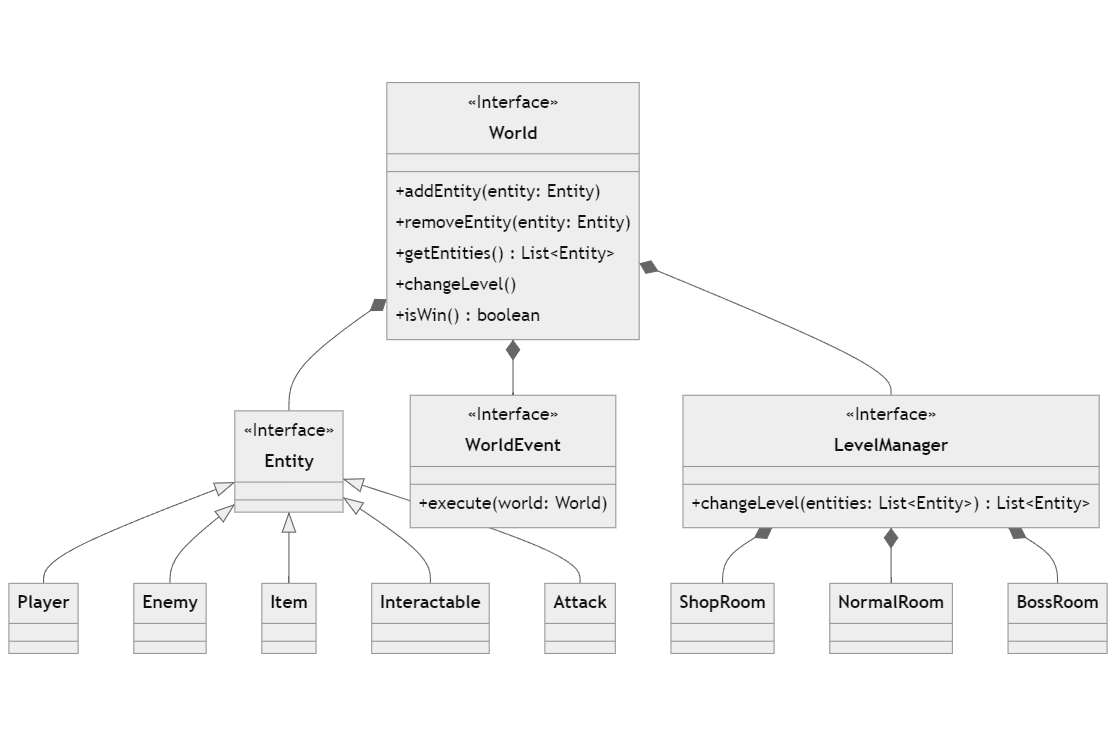
\includegraphics[width=\textwidth]{uml/uml_analisi.png}
	\caption{Diagramma UML dell'analisi del dominio rappresentante le varie entita' di gioco e i loro legami con il mondo e i livelli}
\end{figure}


\chapter{Design}


\section{Architettura}
Abbiamo deciso di utilizzare per il modello del gioco una versione semplificata del \textit{pattern entity-component-system} (\textit{ecs}) mantenendo la parte grafica separata.

Dopo aver tentato un approccio piu' orientato alle gerarchie di classi, ci e' sembrato naturale spostarci verso una visione che fattorizzasse gli aspetti comuni dei diversi attori in gioco in modo piu' modulare, cercando di separare i \textit{dati} (\textit{component}) dalla \textit{logica} che li comanda (\textit{system}).

Questo pattern ci e' sembrato piu' adatto a modellare il nostro gioco perche' supporta la facile creazione di nuovi attori (ad esempio nuovi oggetti, nemici ecc.) garantendo una buona suddivisione del codice e delle responsabilita', un alto riuso e un alto grado di composizione (\textit{composition over inheritance}). 





Di seguito spieghiamo le varie parti della nostra architettura:
\begin{itemize}
	\item \texttt{Component}: sono oggetti utili a mantenere i dati che descrivono un certo aspetto del modello di gioco (ad esempio la posizione, il movimento, il corpo ecc.) e in teoria non hanno una loro logica di comportamento.
	\item \texttt{Entity}: sono dei raccoglitori di \texttt{Component}. Ogni entita' e' descritta dai suoi componenti che permettono alla stessa di distinguerla dalle altre entita'. Ad esempio, diverse entita' presenti in gioco nello stesso momento potrebbero contenere un PositionComponent, un MovementComponent, un BodyComponent, un HealthComponent e altri, che ne descrivono le proprieta'.
	\item \texttt{GameSystem}: sono la parte dell'architettura che si occupa di operare sulle entita', modificandone i componenti e quindi svolgendo la maggior parte della logica del gioco. L'esecuzione sequenziale di vari sistemi, ciascuno che processa le entita' operando su un determinato insieme di componenti, permette il funzionamento del gioco. Ad esempio, il MovementSystem opera esclusivamente sulle entita' che contengono il MovementComponent e si occupa di muovere tutte le entita'; invece, il CheckHealthSystem si occupa di prendere tutte le entita' che hanno un HealthComponent e di rimuovere quelle che hanno esaurito le vite.
	\item \texttt{Engine} e \texttt{World}: queste sono le classi che controllano effettivamente lo svolgersi del gioco. \texttt{Engine} si occupa di gestire il \textit{game loop}, mentre il \texttt{World} contiene al suo interno le entita', esegue i \textit{system} e passa alla View le informazioni necessarie per disegnare su schermo.
	\item \texttt{LevelManager}: manager dei livelli contenuto nel \texttt{World}, che si occupa della generazione e del caricamento degli stessi.
	\item \texttt{View}: e' gestita in modo indipendente dal \textit{pattern ecs}. \texttt{Scene} si occupa solamente di disegnare lo stato del modello di gioco, mentre \texttt{MainWindow} gestisce diverse schermate di menu (home, opzioni, pausa ecc.). Inoltre sono presenti classi che si occupano di disegnare l'interfaccia grafica e di registrare gli input da mouse e tastiera.
\end{itemize}

\begin{figure}[]
	\centering
	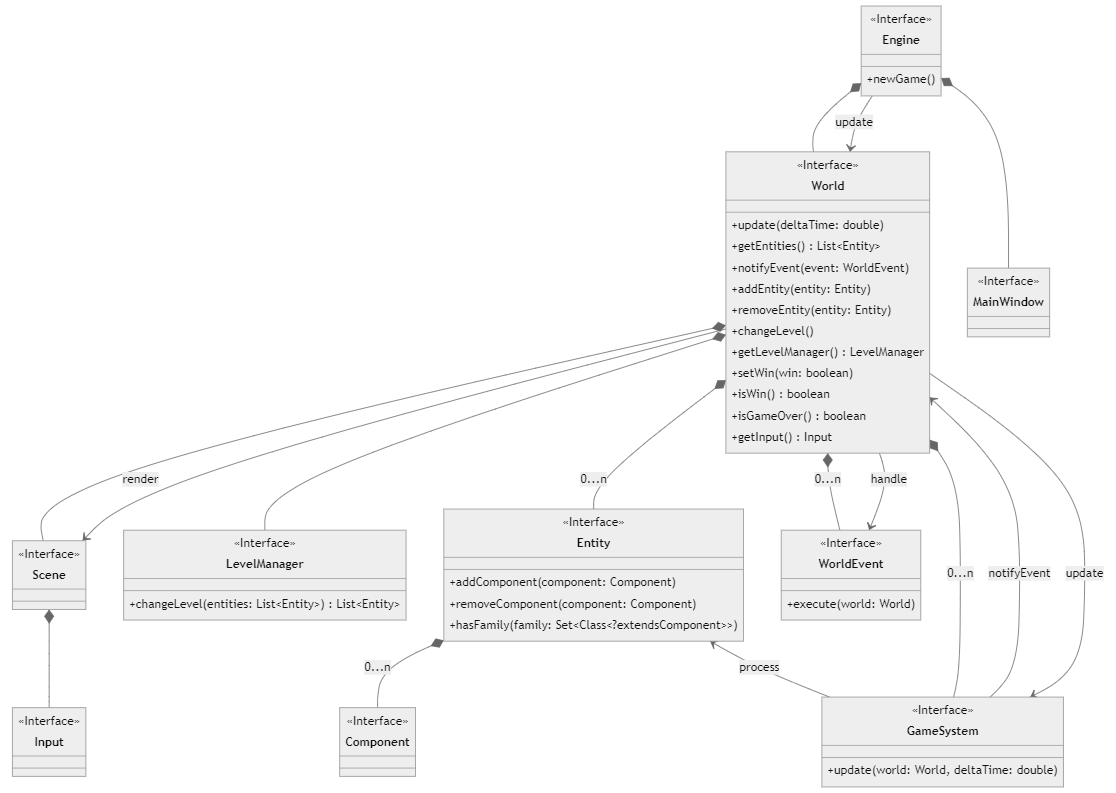
\includegraphics[width=\textwidth]{uml/uml_architettura.png}
	\caption{Diagramma UML dell'architettura. Le freccie indicano le operazioni ad alto livello che le varie parti svolgono. L'\texttt{Engine} fa partire il \textit{game loop} e aggiorna il \texttt{World}, che a sua volta aggiorna uno dopo l'altro tutti i \texttt{GameSystem}. I sistemi processano le entita' che competono alla loro gestione e possono notificare dei \texttt{WorldEvent} al \texttt{World}. Il \texttt{World}, dopo aver eseuguito tutti gli eventi generati dai sistemi, comanda a \texttt{Scene} di disegnare il mondo di gioco}.
\end{figure}

\pagebreak

\section{Design dettagliato}

\subsection{Lorenzo Prati}

Seguendo un approccio bottom-up, di seguito spiego prima il funzionamento della base del \textit{pattern entity-component-system} (\textit{ecs}), per poi passare alla descrizione delle classi fondamentali su cui si poggia il funzionamento dell'applicazione, come Engine e World, e infine dedicarmi ai sistemi e componenti specifici da me realizzati.

\subsubsection{Entity e Component}

\begin{figure}[h]
	\centering
	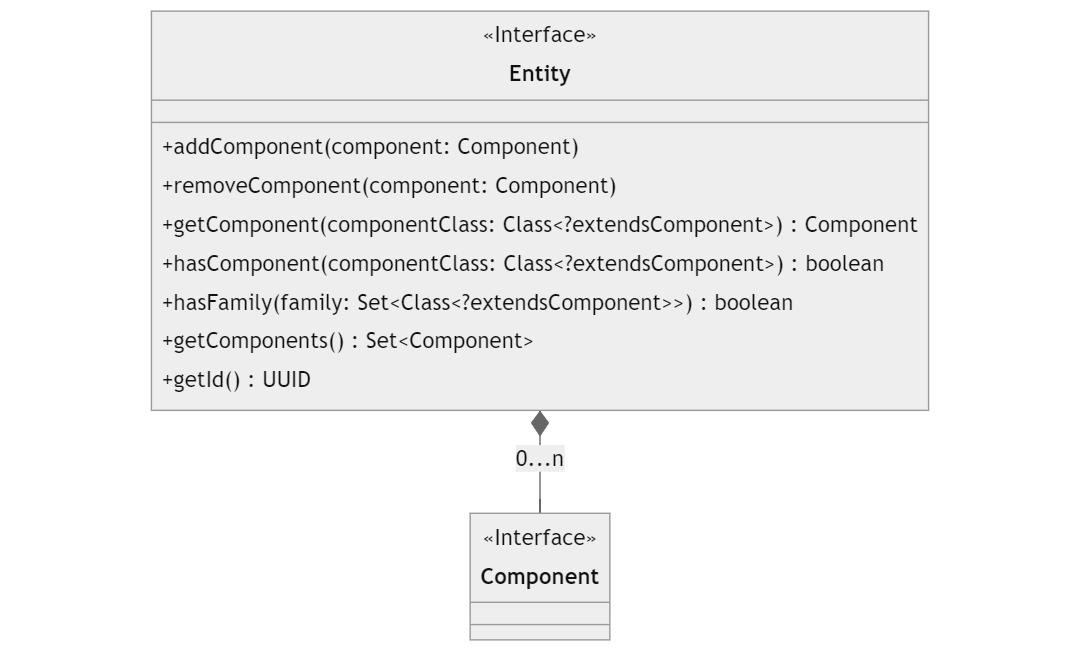
\includegraphics[width=\textwidth]{uml/uml_entity_component.png}
	\caption{Diagramma UML della relazione tra Entity e Component}
	\label{img:badarch}
\end{figure}

\paragraph{Problema}
Modellare il concetto di \textit{entity'} nel contesto del \textit{pattern ecs}. Ogni entita' deve fare riferimento a dei \textit{component} ma non avere una propria logica di comportamento. I componenti devono contenere il piu' possibile solo \textit{dati}. Le entita' devono essere interrogabili sui loro componenti, supportare l'inserimento e la rimozione di componenti, e restituire i componenti richiesti. Nel dominio del gioco, le entita' sono, ad esempio, il giocatore, i nemici, gli oggetti, ma anche gli attacchi.

\paragraph*{Soluzione}
Differentemente dall'approccio classico utilizzato per il \textit{pattern ecs}, che consiste nel rappresentare il concetto di entita' come \textit{id} numerici (interi di fatto) attraverso i quali identificare i vari component, ho scelto di usare un approccio piu' semplice e piu' \textit{object-oriented}, oggetto del corso, realizzando le entita' come classi di tipo \texttt{Entity} contenenti un insieme di \texttt{Component}. Ciascuna entita' possiede comunque un \textit{id} ma questo e' usato in minima parte e solo per esigenze di gestione che esulano da questo paragrafo e che spieghero' in seguito. 
Il vantaggio di questo approccio \textit{oop} e' sicuramente nella semplicita' di gestione; infatti liste di entita', ciascuna con relativo insieme di componenti, sono facilmente iterabili e manipolabili all'occorrenza. Di contro, un approccio piu' a basso livello che favorisca l'uso massiccio di \textit{id} e array di componenti avrebbe permesso un notevole incremento delle performance che pero' e' fuori dallo scopo del progetto.

Quindi, l'interfaccia \texttt{Component} non ha metodi, e serve a essere implementata da tutti i componenti del gioco.
L'interfaccia \texttt{Entity}, invece, contiene tutti i metodi fondamentali per manipolare i componenti contenuti in quell'entita', come ad esempio l'aggiunta e la rimozione, e l'ottenimento di uno specifico componente. Tramite il metodo \texttt{hasFamily} e' possibile interrogare l'entita' sul possesso di un insieme di \texttt{Component} specifici, cosa che risultera' molto utile per i \textit{system}.

Su queste semplici interfacce si basa l'intera struttura del \textit{pattern entity-component-system}, o meglio della parte \textit{entity-component}.

Infine, ho realizzato una classe \texttt{EntityBuilder} che, tramite l'uso del \textit{builder pattern}, consente la creazione di entita' in modo dichiarativo semplicemente tramite l'aggiunta sequenziale di \texttt{Component} su cui si basano tutte le factory presenti nel progetto. Per creare nuove entita' e' quindi sufficiente aggiungere componenti tramite l'\texttt{EntityBuilder} e modificando i parametri di creazione di questi componenti oppure creandone di nuovi, e' di fatti possibile creare molto velocemente nemici, oggetti e attacchi nuovi e dalle caratteristiche diverse.

Un esempio di creazione di entita' sfruttando il builder e il \textit{pattern factory method} da me realizzato: (inserire permalink)

\subsubsection{System}

\begin{figure}[h]
	\centering
	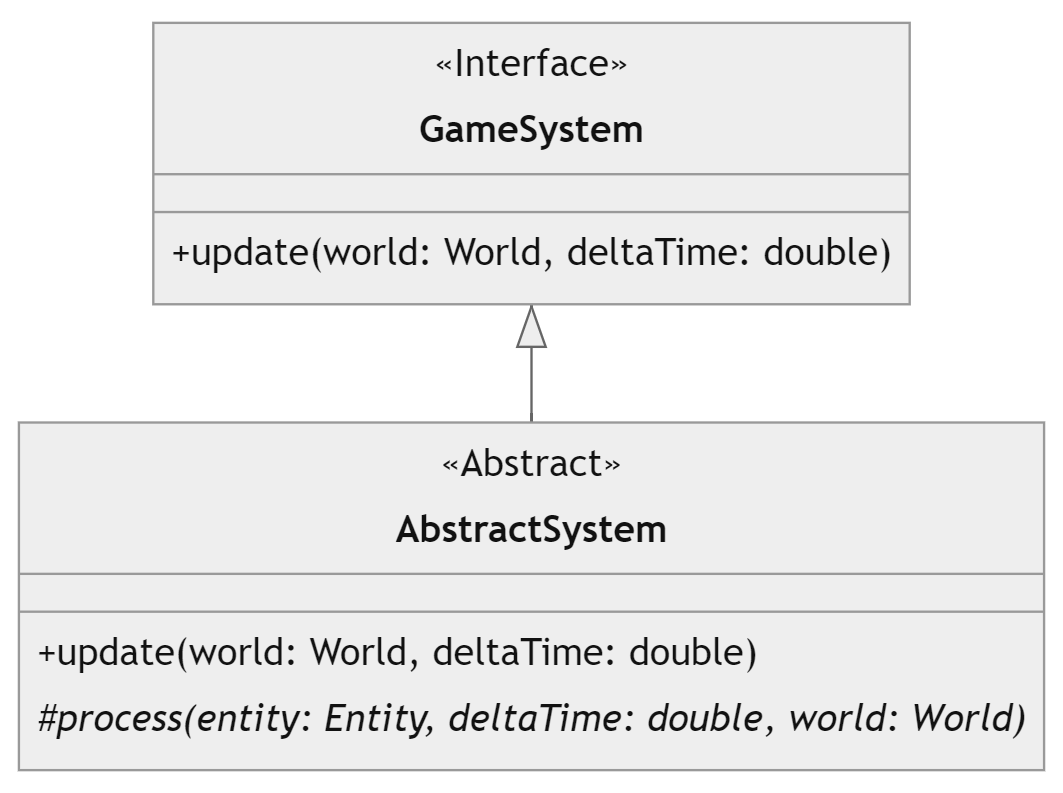
\includegraphics[width=\textwidth]{uml/uml_system.png}
	\caption{Diagramma UML dei \textit{system}} 
\end{figure}

\paragraph{Problema}
Le entita' e i componenti non definiscono logica di comportamento propria, quindi e' necessario che vengano manipolati dai \textit{system}. I sistemi devono essere divisi per specifico compito e ognuno deve essere in grado di operare sulle entita' che hanno certi componenti. Ad esempio, devono essere realizzati dei sistemi in grado di muovere le entita', rilevare e gestire le loro collisioni, rimuoverle dal mondo di gioco quando necessario ecc.

\paragraph[]{Soluzione}
Ho realizzato un'interfaccia \texttt{GameSystem} che modella un generico \textit{system}. Il metodo esposto e' \texttt{update} e si occupa di far eseguire la logica del sistema. Visto che ogni \textit{system} deve essere in grado di operare solo su certe entita', per garantire il \textit{riuso} ho scelto di realizzare una classe astratta \texttt{AbstractSystem} che all'interno utilizza il \textit{pattern template method} dove il metodo template e' appunto \texttt{update}, che fa i dovuti controlli sui componenti che compongono l'entita' e poi richiama il metodo astratto e protetto \texttt{process} solo sulle entita' che hanno i componenti richiesti. In questo modo, ogni classe che estende \texttt{AbstractSystem} deve solamente occuparsi di definire tramite costruttore l'insieme di \texttt{Component} su cui vuole operare e poi implementare il metodo \texttt{process} che andra' ad operare solo su \texttt{Entity} che hanno i componenti precedentemente richiesti.

I \textit{system} sono in grado, avendo nel loro metodo \texttt{process} un riferimento al \texttt{World}, di notificare, come spieghero' meglio in seguito, degli eventi; ma e' anche possibile un metodo di \textit{signaling} tra \textit{system} diversi. Questo e' possibile attaccando, in seguito al verificarsi di una determinata situazione, un componente \textit{informativo} all'entita' che si sta processando in modo tale da permettere a successivi \textit{system} di cercare entita' con quel componente \textit{informativo} e gestire la cosa adeguatamente.

In teoria e' quindi sufficiente, per inserire nel gioco una nuova meccanica, costruire nuovi componenti che definiscano nuove proprieta' e un nuovo sistema che operi su di essi senza il bisogno di andare a modificare i sistemi o i componenti precedentemente creati.

\subsubsection{Engine}

\begin{figure}[h]
	\centering
	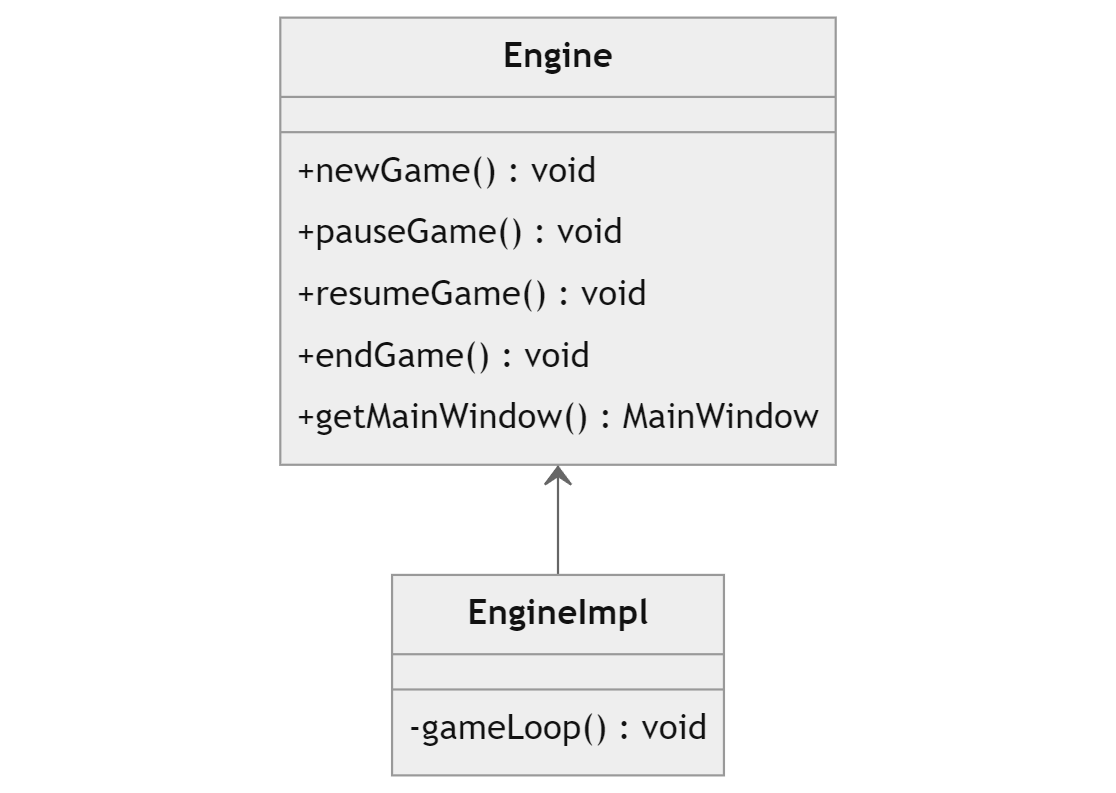
\includegraphics[width=\textwidth]{uml/uml_engine.png}
	\caption{Diagramma UML dell'Engine}
	\label{img:badarch}
\end{figure}

\paragraph*{Problema}
Realizzare una classe che permetta lo svolgimento effettivo del main loop del gioco, attraverso il quale scandire gli update del modello e della rappresentazione grafica, e che contenga tutti gli elementi per mantenere attiva l'applicazione. All'occorrenza, deve anche essere possibile mettere in pausa il gioco e riprenderlo. Deve essere inoltre gestita la fine del gioco.

\paragraph*{Soluzione} La soluzione e' ricaduta sulla creazione di un'interfaccia \texttt{Engine} con relativa implementazione \texttt{EngineImpl}. Questa classe fa uso del \textit{pattern game loop}, realizzato in un metodo privato, e vengono esposti dall'interfaccia i metodi necessari alle altre classi (ad esempio le schermate della View) per controllare il loop. E' quindi possibile metterlo in pausa, riprenderlo e arrestarlo. Essendo questa classe la prima che viene creata al lancio dell'applicazione, essa si occupa anche internamente di creare il \texttt{World} e \texttt{MainWindow}.

\subsubsection{World e Eventi}

\begin{figure}[h]
	\centering
	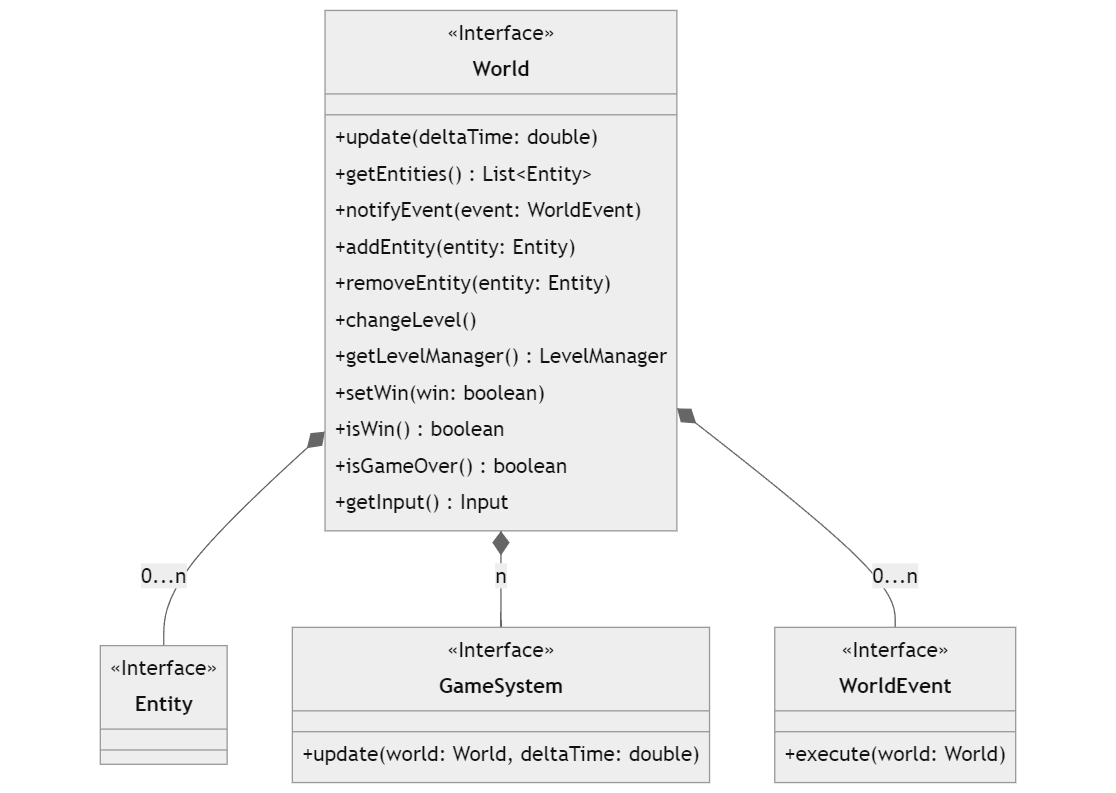
\includegraphics[width=\textwidth]{uml/uml_world.png}
	\caption{Diagramma UML del World}
	\label{img:badarch}
\end{figure}

\paragraph*{Problema}
Occorre contenere e mantenere le \texttt{Entity}, e comandare la logica che opera su di esse, cioe' i \textit{system}. Allo stesso tempo, e' necessario passare alla View le informazioni necessarie affinche' possa disegnare sia le entita' che la mappa di gioco. 

\paragraph*{Soluzione}
Ho scelto di unire in un'unica classe la funzione di contenere le entita' e i sistemi, e la rappresentazione grafica del mondo di gioco (\texttt{Scene}), quindi ho realizzato l'interfaccia \texttt{World} con la relativa implementazone \texttt{WorldImpl}. Ho optato per questa scelta di nome nonostante la funzione della classe sia piu' comparabile a quella di un classico \textit{Controller} del pattern MVC poiche' e' utilizzato spesso nel contesto del \textit{pattern ecs}.

L'interfaccia \texttt{World} espone i metodi necessari al controllo del gioco vero e proprio e delle entita', come ad esempio il metodo \texttt{update}, che viene chiamato ad ogni ciclo del \textit{game loop}. Questo e' il metodo principale della classe, perche' si occupa di:

\begin{itemize}
	\item eseguire tutti i \texttt{GameSystem}, che equivale ad \textit{aggiornare} il modello
	\item eseguire tutti gli eventi in coda nel \texttt{World}
	\item comandare alla scena di disegnare, solo dopo aver passato tramite pacchetti \textit{GraphicInfo} le informazioni necessarie al disegno per ciascuna entita'
\end{itemize}

Ho scelto di memorizzare e gestire i \texttt{GameSystem} direttamente in una lista dentro il \texttt{World} per semplicita' quando di fatti l'ordine con cui essi vengono memorizzati nella lista e quindi eseguiti ad ogni ciclo di \textit{update} potrebbe essere gestito da uno \textit{strategy pattern} ed essere modificabile in futuro con un'altra implementazione; tuttavia ho scelto di semplificare l'approccio perche' in ogni caso non viene gestita in nessun modo l'abilitazione/disabilitazione di sistemi a run-time (come e' comune nel \textit{pattern ecs}) e in generale in un gioco semplice come il nostro i pochi sistemi presenti devono eseguire strettamente uno dopo l'altro in un certo ordine preciso che di fatti lascia spazio a poche variazioni. Per questi motivi, la gestione dei sistemi e' fissa e non modificabile, e per questo l'inizializzazione dei \texttt{System} e' gestita internamente al \texttt{World} e non e' visibile o modificabile dall'esterno.

Poi il \texttt{World} espone i metodi per la gestione delle \texttt{Entity}, cioe' che permettono di aggiungere e rimuovere \texttt{Entity}, oppure di ottnere una copia delle entita' presenti in gioco.

Gli eventi sono rappresentati tramite l'interfaccia \texttt{WorldEvent} e sono gestiti in modo asincrono. Durante la loro esecuzione, i vari \textit{system} possono notificare il \texttt{World} di uno specifico evento, che verra' messo in una coda ed eseguito solo dopo che tutti i \texttt{System} hanno finito la loro esecuzione. In questo modo si evita il verificarsi di comportamenti anomali dovuti all'immissione di \texttt{Entity} nel \texttt{World} nel mezzo dell'esecuzione dei \textit{system} durante la quale, d'altra parte, e' risultato comodo sia immettere che rimuovere le \texttt{Entity} tramite eventi dedicati, in modo da reagire all'aggiunta/eliminazione di una specifica entita' (ad esempio per il \textit{game over}). Mi sono occupato io di implementare tutti gli eventi, che saranno pero' lanciati anche dai \textit{system} realizzati dai miei colleghi:
\begin{itemize}
	\item \texttt{AddEntityEvent} aggiunge l'entita' passata come parametro al \texttt{World}
	\item \texttt{RemoveEntityEvent} rimuove dal \texttt{World} l'entita' passata come parametro, in questo caso identificata tramite \textit{id}. Nel caso si trattasse dell'entita' che rappresenta il giocatore o il boss, viene notificato il \texttt{World} rispettivamente della sconfitta o della vittoria
	\item \texttt{ChangeLevelEvent} chiama il metodo \texttt{changeLevel()} del \texttt{World}, che procede a gestire il cambio di livello aggiornando le entita' con quelle generate dal \texttt{LevelManager} per il nuovo livello e passando a \texttt{Scene} anche la nuova mappa.
\end{itemize}

Il \texttt{World} espone anche un metodo per ottenere la classe con la quale i \texttt{System} possono sfruttare l'input dell'utente, che spieghero' piu' nel dettaglio descrivendo il funzionamento del giocatore.

Infine, sono presenti vari metodi che servono a interrogare il \texttt{World} sullo stato della partita
(\texttt{isGameOver()}) e il risultato della partita (\texttt{isWin()}), utili soprattutto all'\texttt{Engine} che deve sapere quando arrestare il \textit{game loop} e gestire la fine del gioco.

\subsubsection{Movimento e Posizione}

\begin{figure}[h]
	\centering
	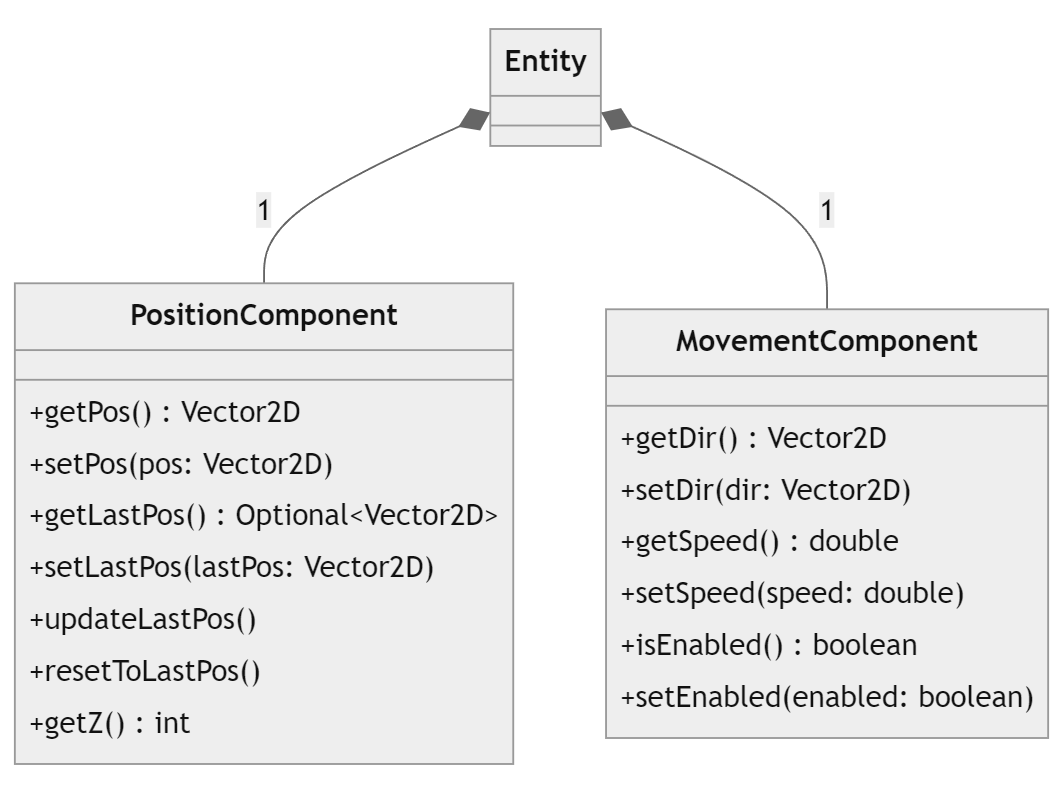
\includegraphics[width=\textwidth]{uml/uml_pos_mov.png}
	\caption{Diagramma UML dei componenti della posizone e del movimento}
\end{figure}

\paragraph{Problema}
Tutte le entita' di gioco occupano una posizione nella mappa di gioco, che a livello di modello possiamo rappresentare come un piano 2d. Mentre alcune entita' mantengono la loro posizione invariata nel tempo (come gli item), altre (come i nemici e il giocatore) variano la posizione nel tempo muovendosi in diverse direzioni secondo le logiche dell'intelligenza artificiale o un input dell'utente.

\paragraph{Soluzione}
Ho realizzato una classe \texttt{PositionComponent} che ovviamente implementa l'interfaccia \texttt{Component} e memorizza le coordinate della posizione di un'entita' in quel momento. Inoltre, al suo interno viene memorizzata anche la posizione precedente a quella corrente, poiche' sara' utile nel momento di gestire le collisioni. La posizione viene quindi memorizzata come dato all'interno del componente, cosi' da poter attaccare ad ogni entita' (tutte di fatto) che hanno una posizione nella mappa un \texttt{PositionComponent}, massimizzando il \textit{riuso di codice}. 

Analogamente, per rappresentare il movimento ho creato un componente \texttt{MovementComponent}, che memorizza la direzione in cui il movimento deve essere compiuto, tramite un vettore 2d. Inoltre, viene qui memorizzata anche la velocita' con la quale l'entita' dovra' compiere il movimento. Il movimento puo' anche essere abilitato/disabilitato. La scelta di gestire il movimento tramite vettori, nonostante le entita' di gioco si muovano quasi tutte soltanto nelle 4 direzioni, permette in futuro anche la facile implementazione del movimento nelle 8 direzioni, o comunque una sua gestione libera.

Una volta definiti questi componenti di base, e' possibile gestire il movimento di tutte le entita' tramite un \textit{system}. Il \texttt{MovementSystem} si occupa infatti di processare le entita' che hanno un componente \texttt{MovementComponent}, che significa che \textit{posseggono la capacita' di muoversi e hanno i dati necessari affinche' possano essere mosse}, e si occupa di verificare per ciascuna di queste entita' se il movimento e' abilitato e nel caso aggiornare il \texttt{PositionComponent} con la nuova posizione risultante dal calcolo del movimento espresso nel \texttt{MovementComponent} applicato alla vecchia posizione. L'esecuzione di questo \textit{system} ad ogni ciclo del \textit{game loop}, permette di muovere tutte le entita' che \textit{possono farlo} previo precedente settaggio della direzione in cui l'entita' intende muoversi.

\subsubsection{Collisioni e fisica}

\begin{figure}[h]
	\centering
	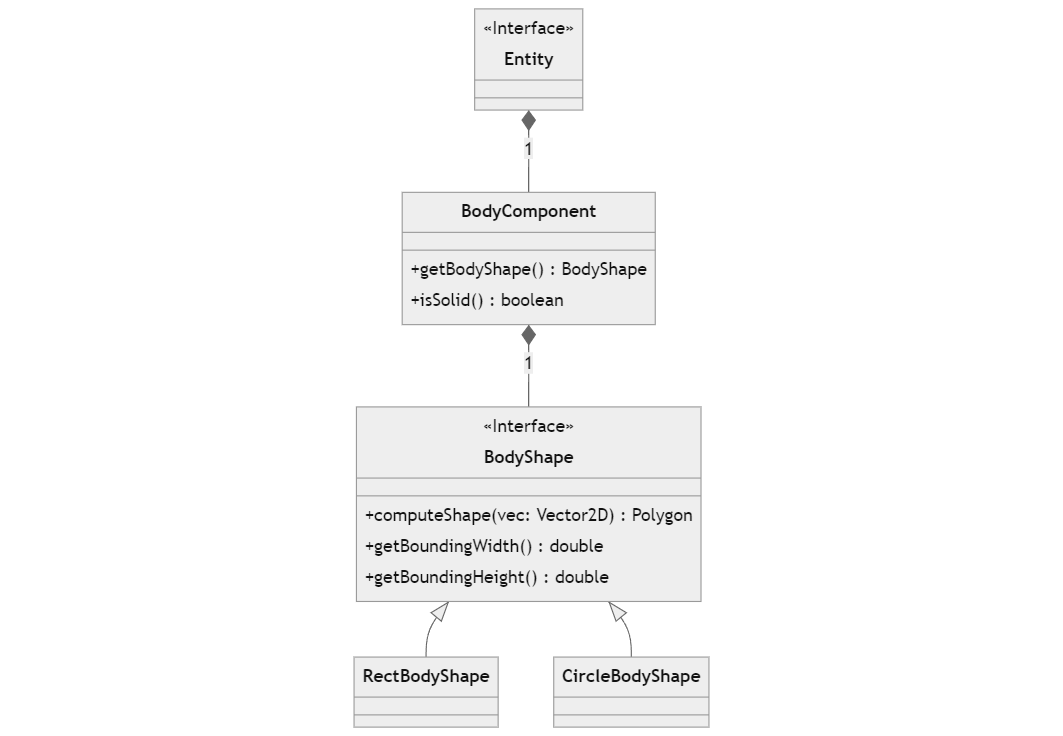
\includegraphics[width=\textwidth]{uml/uml_body.png}
	\caption{Diagramma UML del componente del corpo e delle shape}
\end{figure}

\paragraph{Problema}
Alcune entita' hanno corpi \textit{solidi} e devono comportarsi come tali nelle loro azioni di movimento. Inoltre e' necessario registrare quando entita' di qualunque tipo collidono con altre entita', al fine di poterne gestire le conseguenze.

\paragraph{Soluzione}
Ho realizzato una classe \texttt{BodyComponent} che modella il \textit{corpo} di un'entita', definendone proprieta' come la \texttt{BodyShape}, ovvero la forma geometrica che il suo corpo occupa nello spazio, e la solidita'
(espressa da un booleano). 

Il \texttt{CollisionSystem} si occupa di processare le entita' che hanno un \texttt{BodyComponent}. Per ciascuna di queste entita', viene controllata la collisione con \textit{tutte} le altre entita' presenti nel gioco. Se viene rilevata una collisione, calcolata estrendo dai rispettivi \texttt{BodyComponent} le body shape e controllandone l'intersezione in date coordinate, allora viene \textit{registrata} la collisione attaccando all'entita' che il system sta processando in quel momento un \texttt{CollisionComponent}, un semplice componente che mantiene i dati sulle collisioni avvenute. In particolare, viene aggiunto un \texttt{CollisionComponent} solo nel caso non ce ne sia gia' uno, poiche' altrimenti vengono aggiornate le informazioni di quello gia' presente aggiungendo i dati sulla nuova collisione. Questo e' un esempio, l'unico in realta' realmente presente in questo progetto, di \textit{signaling tra system}. Infatti, i successivi \textit{system} potranno filtrare le entita' che hanno tra i loro componenti anche un \texttt{CollisionComponent} e gestire la collisione in modo appropriato. Su questo meccanismo si basano i sistemi che gestiscono le collisioni fisiche, gli item, il combattimento ecc. poiche' la loro gestione si basa sulla precedente aggiunta di un \texttt{CollisionComponent} da parte del \texttt{CollisionSystem}.

Un \texttt{PhysicsSystem}, che esegue subito dopo il \texttt{CollisionSystem}, processa le entita' che hanno \texttt{BodyCompoenent} e \texttt{CollisionComponent} occupandosi invece della gestione vera e propria della collisione fisica, che pero' nel dominio del gioco si traduce in un semplice reset della posizione. Dato che vengono tenute nel \texttt{PositionComponent} sia la posizione corrente che quella immediatamente passata, solo in caso di collisione tra corpi \textit{solidi} viene ripristinata la posizione precedente.

Menziono qui anche la presenza di un \texttt{ClearCollisionSystem}, un semplice sistema che esegue dopo che hanno eseguito tutti i sistemi che dovevano in qualche modo gestire la reazione a una collisione (filtrando anche per \texttt{CollisionComponent}), rimuovendo tutti i \texttt{CollisionComponent} dalle entita' che ne hanno uno. In questo modo, al successivo loop di update dei system, non vengono lasciate collisioni non gestite.

Per quanto riguarda infine l'interfaccia \texttt{BodyShape}, essa puo' essere implementata potenzialmente da classi che rappresentano varie forme geometriche. Io ho realizzato una \texttt{RectBodyShape}, che rappresenta la forma geometrica del rettangolo, e una \texttt{CircleBodyShape}, che rappresenta il cerchio. L'interfaccia espone il metodo \texttt{computeShape(Vector2D)} che permette di ricevere il poligono calcolato in base alle coordinate fornite, utile poi al calcolo dell'intersezione con un altro poligono. Qui ho fatto uso di libreria come spiegato meglio nel paragrafo dedicato (riferimento). Inoltre, sono presenti i metodi \texttt{getBoundingWidth()} e \texttt{getBoundingHeight()} per conoscere il rettangolo che limita il poligono, utili sia alla View che in altri punti del progetto.

\newpage

\subsubsection{Logica del giocatore e Input}

\begin{figure}[h]
	\centering
	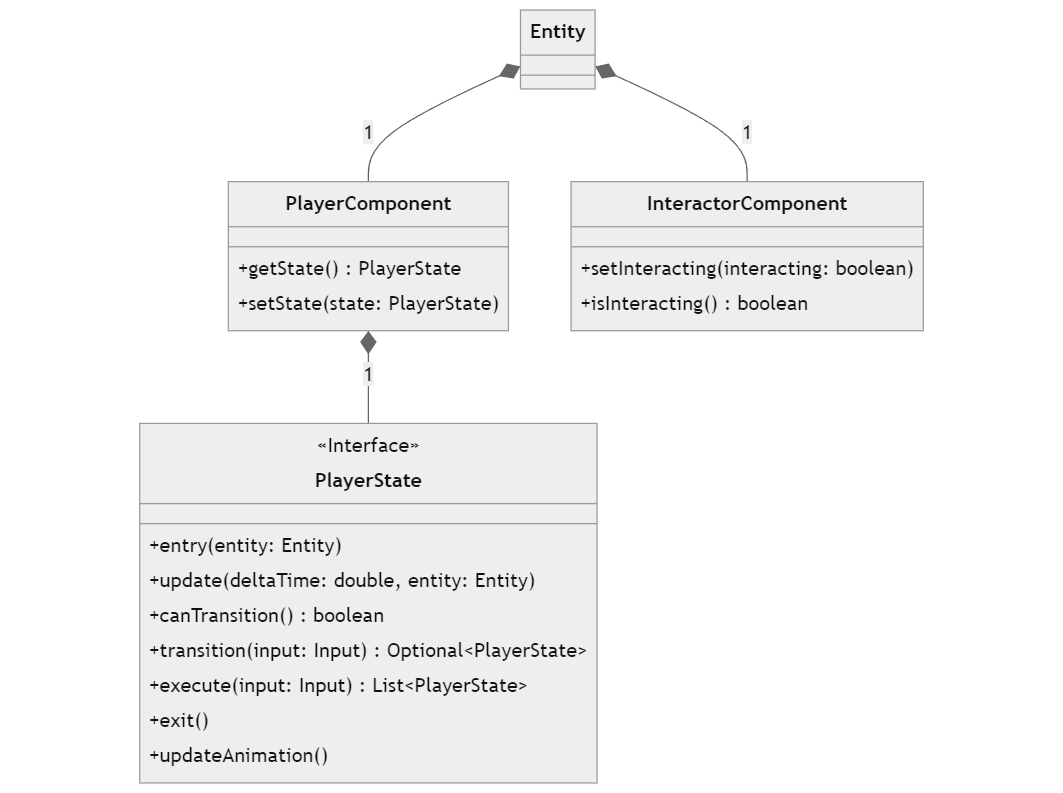
\includegraphics[width=\textwidth]{uml/uml_player.png}
	\caption{Diagramma UML dell'entita' che rappresenta il giocatore e alcuni dei suoi componenti}
\end{figure}

\paragraph{Problema}
L'utente controlla un personaggio in grado di:

\begin{itemize}
	\item muoversi in 4 direzioni (su, giu', destra, sinistra)
	\item attaccare con la spada
	\item sparare un proiettile
	\item caricare una palla di fuoco e spararla rilasciando il tasto
	\item interagire con oggetti
\end{itemize}

Ognuna di queste azioni e' rappresentata a schermo da un'animazione differente. Alcune di queste azioni hanno condizioni per poter essere eseguite, oppure possono essere eseguite solo dopo aver compiuto altre azioni; ma in ogni momento il giocatore esegue solo una di queste azioni.

\paragraph{Soluzione}
Ho risolto il problema utilizzando lo \textit{state pattern} in combinazione con un \texttt{PlayerInputSystem}. Infatti, se abbiamo cercato di rispettare il pattern \textit{ecs} il piu' possibile, specialmente cercando di gestire la logica di comportamento delle entita' interamente nei \textit{system} quando possibile, si e' convenuto che non abbia senso forzarlo su ogni aspetto, percio' in questo e in altri casi parte della logica e' stata spostata fuori dai system cercando di semplificare l'aspetto del \textit{behaviour} presente in alcune implementazioni dell'\textit{ecs}. 

In questo caso, il giocatore e' un entita' come le altre, definita dall'insieme dei suoi componenti. Il componente che lo distingue maggiormente pero' e' il \texttt{PlayerComponent}, che non contiene lui stesso la logica del comportamento del player, ma contiene delle classi che hanno questa logica, cioe' gli \textit{stati} del player (\texttt{PlayerState}). 

Il \texttt{PlayerInputSystem}, che e' il primo \textit{system} a eseguire nel gioco ad ogni loop, processa le entita' che hanno un \texttt{PlayerComponent} (lasciando quindi aperta la possibilita' di gestire piu' giocatori). Per semplicita' di spiegazione, assumiamo che l'entita' che rappresenta il giocatore sia una sola. In questo caso, tale entita' viene processata normalmente dal sistema, che ne gestisce il \textit{cambio di stato} in base all'input dell'utente agendo come parte di una \textit{finite state machine}.

\begin{figure}[h]
	\centering
	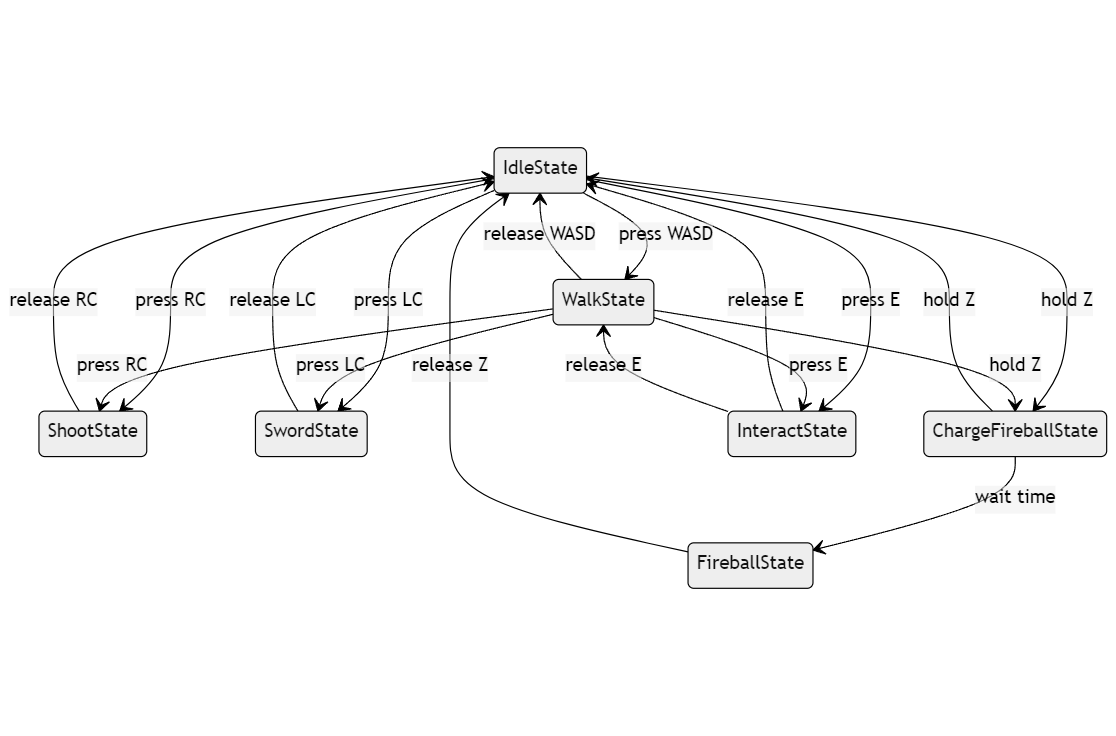
\includegraphics[width=\textwidth]{uml/player_states.png}
	\caption{Diagramma degli stati del player. LC ed RC indicano rispettivamente il tasto sinistro e destro del mouse. Il player puo' trovarsi solo in uno di questi stati alla volta} 
\end{figure}

Il \texttt{PlayerComponent} contiene lo \textit{stato} corrente in ogni momento, quindi viene estratto tale \texttt{PlayerState} e interrogato sulla possibilita' di poter effettuare un cambio di stato in base all'\texttt{Input}; se possibile, quindi, il \texttt{PlayerState} corrente restituisce il prossimo stato calcolato sempre sulla base dell'input e il system procede con la transizione di stato, sostituendo lo stato corrente nel \texttt{PlayerComponent} con il nuovo stato calcolato. Se lo stato corrente puo' transitare, allora viene anche chiamato il metodo \texttt{execute}, che potrebbe generare nuove entita', ad esempio proiettili o attacchi, e queste vengono poi aggiunte al \texttt{World} tramite evento. Il cambio di stato piu' nel dettaglio e' gestito dai metodi \texttt{entry} ed \texttt{exit} che gestiscono rispettivamente le operazioni da effettuare nei due momenti per quello stato. Infine, il system aggiorna l'animazione (vedi spiegazione animazioni). 

Ciascuno stato estende una classe \texttt{AbstractState} che fattorizza alcuni metodi dell'interfaccia \texttt{PlayerState} come \texttt{canTransition()} (che si occupa di controllare che lo stato non sia bloccato in un animazione non cancellabile), \texttt{update(double, Entity)} (che si occupa soprattutto di aggiornare il tempo passato nello stato) e altri che sono utili alle sottoclassi come \texttt{setAnimationState(String)}. Inoltre, vengono fornite delle implementazioni di default dei metodi d'interfaccia \texttt{entry(Entity), \texttt{exit()}} e \texttt{execute(Input)}, overridabili a piacimento dalle sottoclassi per definire comportamenti piu' complessi. Invece, il metodo \texttt{transition(Input)} e' lasciato astratto da implementare per ogni singolo stato poiche' ognuno definisce logiche proprie di transizione verso altri stati, che non descrivo nei dettagli poiche' credo gia' sufficiente esplicate nel diagramma sopra. Infine, ogni stato implementa il metodo \texttt{updateAnimation()} settando una specifica animazione.

Di seguito gli stati:
\begin{itemize}
	\item \texttt{IdleState} rappresenta lo stato di \textit{idle}, cioe' in cui il giocatore e' fermo, e si occupa solo di disabilitare il movimento in entrata.
	\item \texttt{WalkState} rappresenta lo stato di camminata, e si occupa di abilitare/disabilitare il movimento in entrata/uscita e di settare la direzione del \texttt{MovementComponent} coerentemente con l'input dell'utente.
	\item \texttt{SwordState} rappresenta lo stato di attacco ravvicinato, che si occupa di restituire l'entita' che rappresenta l'attacco ravvicinato, tramite relativa factory
	\item \texttt{ShootState} rappresenta lo stato di attacco dalla distanza, che si occupa di restituire l'entita' che rappresenta il proiettile, tramite relativa factory
	\item \texttt{ChargeFireballState} rappresenta lo stato di carica della fireball, che si occupa di gestire il fatto che si rimanga nello stato fino a quando il giocatore tiene premuto il tasto, ma, se e' passato un certo tempo e solo se il giocatore ha anche rilasciato il tasto, si passa allo stato \texttt{FireballState}
	\item \texttt{FireballState} rappresenta lo stato di attacco dalla distanza con una fireball, che si occupa di restituire l'entita' che rappresenta la fireball, tramite relativa factory
	\item \texttt{InteractorState} rappresenta lo stato in cui il player puo' interagire con oggetti che hanno un \texttt{InteractableComponent} (power up dello shop, gate ecc.); lo stato si occupa solamente di abilitare/disabilitare l' \texttt{InteractorComponent} in entrata/uscita
\end{itemize}

L'interfaccia \texttt{Input} e'ottenibile tramite getter dal \texttt{World} e interrogabile sui tasti premuti dall'utente tramite dei semplici getter; in questo modo i vari stati sono in grado di sapere quali azioni sta attualmente cercando di realizzare l'utente.

Ho realizzato una classe \texttt{InputListener} che, tramite i metodi di Swing, registra l'input da mouse e tastiera e chiama dei setter su un'istanza di \texttt{Input}. Questa istanza viene poi passata al \texttt{World} tramite una copia, garantendo in questo modo ai \textit{system} di gioco di operare con una classe completamente separata dalla View.

\subsubsection{Schermata vittoria/sconfitta}
Ho realizzato anche una schermata di View, cioe' la schermata di vittoria e sconfitta. Qui, tramite il passaggio di un parametro booleano che indica la vittoria/sconfitta, viene semplicemente visualizzata un'immagine di sfondo e un messagio finale differente.


\subsection{Elvis Perlika}
In questa sezione si approfondirà la parte di \textit{AI} dei nemici
ed il \textit{Combat System} tra gli stessi nemici e player.\\
(Tendenzialmente affronterò la descrzione delle soluzioni con un approccio contrario a quello
del mio collega Lorenzo Prati, cioè Top-Bottom)

\subsubsection{AI}

\paragraph{Obbiettivo}
Progettare nemici con caratteristche differenti, in modo
da offrire al giocatore una varietà di situazioni e strategie da affrontare.
Tuttavia, nonostante le differenze tra di loro, l'obbietivo dei nemici deve
rimanere quello di eliminare il giocatore.
\begin{figure}[h]
	\centering
	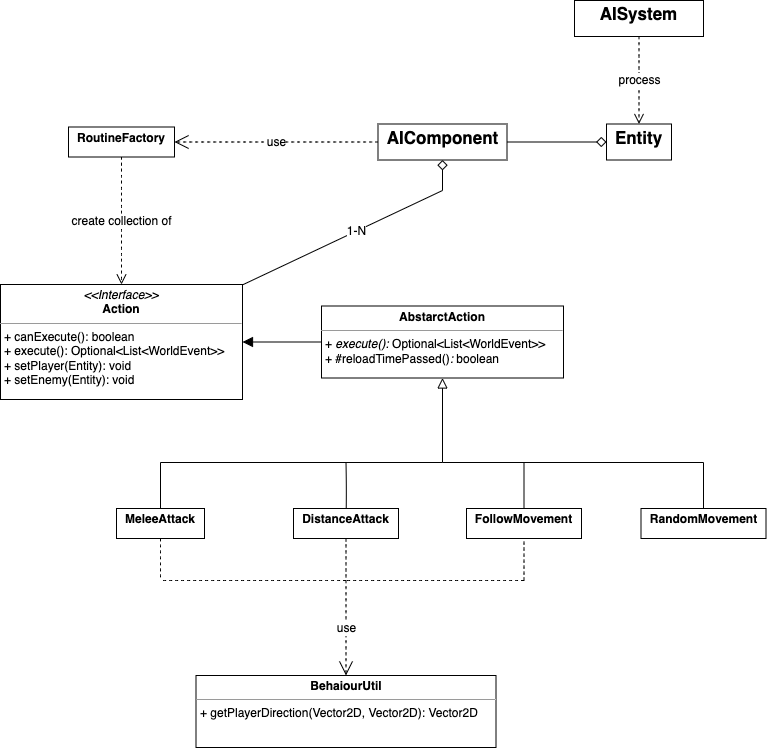
\includegraphics[width=\textwidth]{uml/UML_AI.png}
	\caption{Diagramma UML delle Action.}
	\label{img:badarch}
\end{figure}

\paragraph{Problema}
I nemici devono avere comportamenti diversi.
Per \textit{Comportamento} si intende "Insieme di azioni, di atteggiamenti con cui 
l'individuo esterna la propria personalità, rapportandosi agli altri e all'ambiente".
\paragraph{Soluzione}
Prendendo spunto dal \textit{Pattern Strategy} ho creato l'interfaccia \texttt{Action}.
Nel mio caso però le Action, a differenza del classico \textit{Pattern Stratgy}, 
oltre ad eseguire una certa azione valutano se è il caso di eseguirla.
Data la definizione di \textit{Comportamento} citata prima, per creare comportamenti predefiniti 
ho deciso di implementare la classe \texttt{RoutineFactory} che crea collezioni di azioni 
seguendo il \textit{Pattern Factory Method}.\\

\underline{Esempio:} \textit{createShooterRoutine()} restituisce una classica personalità da zombie:
segue il player se lo rileva nella sua aggro zone, lo attacca se è abbastanza vicino oppure si muove
casualmente nel caso non sia il caso di eseguire le precedenti azioni.

\paragraph{Problema}
Tutte le Action in questa prima versione del gioco presentano una caratteristca comune:
si attivano tenendo conto soltanto della distanza dal player.
\paragraph{Soluzione}
Ho deciso di creare la classe astratta \texttt{AbstractAction} che implementa il metodo \textit{canExecute()} il quale 
valuta la distanza tra AI e giocatore. Oltre a quel metodo ho sfruttto la classe astratta per fattorizzare altri metodi comuni.
E' nota la limitazione che questo sistema provoca ma si è deciso che per un gameplay semplice come il nostro
potesse comunque andare bene.

\paragraph{Problema}
Permettere alle Action di creare nuove entità, ad esempio: attacchi.
\paragraph{Soluzione}
Per creare nuovi attacchi performati dalle AI nemiche ho creato la classe \texttt{EnemyAttackFactory} seguendo il 
\textit{Pattern Factory Method}.\\

\underline{Nota:} Per distinguere gli attachi da altre entità ho creato l'\texttt{AttackComponent}.
L'\texttt{AttackComponent} mantiene anche i dati relativi al danno del attacco.\\

Ho quindi deciso di far restituire dal metodo \textit{execute()}, presente nelle \texttt{Action}, una 
lista opzionale di \texttt{WorldEvent} che l'\texttt{AISystem} si occuperà di notificare al \texttt{World}.
In una Action utile per attaccare sarà logico restituire una lista con eventi di tipo \textit{AddEntityEvent}
che prendono come parametro entità create dalla \texttt{EnemyAttackFactory}.

\paragraph{Problema}
La classi utili alla creazione di attacchi come \texttt{EnemyAttackFactory} oppure \texttt{PlayerAttackFactory}
hanno metodi comuni utili al corretto posizionamento e direzionamento degli attacchi.
\paragraph{Soluzione}
Ho fattorizzato i metodi comuni in una classe astratta \texttt{AbstractAttackFactory}.
Non ho fatto lo stesso per il metodo \textit{getPlayerDirection()} che permette alle
AI di rintracciare il player perché ha la sua utilità sia in Action di attacco che non;
quindi ho inserito il metodo nella classe \texttt{BehaviourUtil}. 

\paragraph{Conclusione}
Ho ideato quindi un sistema che permette di creare nuove \texttt{Action} basandosi sullo spazio 
intorno alla AI e sullo scorrere del tempo. 
Considerato il dominio di gioco semplice, nonostante le chiare litazione che questo sistema presenta, 
riesce, nel suo piccolo, nella creazione di nuove personalità.
Nelle sezione precedenti ho trattato soltanto di AI nemiche ma questo sistema
permette anche la creazione di AI assegnabili ad NPC.

\subsubsection{Combat System}

\paragraph{Problema}
Evitare che le AI nemiche causino danno a loro AI alleate.
\paragraph{Soluzione}
Ho sfruttato lo stesso sistema ideato dalla collega Alessandra Versari 
per la creazione degli Item.\\
Per dettagli referenzio alla sezione di Design Dettagliato 
della collega.

\subsubsection{HUD}

\paragraph{Problema}
Creare un HUD semplice che mostri vita e monete del giocatore.
\paragraph{Soluzione}
Avrei potuto costruire un HUD più modulare ma dato il nostro dominio di 
gioco semplice ho valutato che bastassero pochi semplici metodi per la 
visualizzazione del HUD. 

\subsection{Emanuele Dajko}








\subsection{Alessandra Versari}
\subsubsection*{Items}
\paragraph*{Problema}
	Con item si intende un oggetto di gioco che verrà raccolto a seguito del passaggio del player sopra ad esso. Gli item presenti nel nostro gioco sono cuori e monete.
	Ciascun item una volta entrato in contatto con un'entità deve prima verificare che si tratti del player ed effettuare i controlli necessari prima di applicare il proprio “effetto” (cioè la conseguenza/reazione che l'item avrà sull'entità che ha colliso con esso).
	Di seguito le principali caratteristiche degli items presenti nel nostro gioco:
	\begin{itemize}
		\item Gli items “cuore” permetteranno di aumentare la vita corrente del player, ma ciò verrà fatto solo a seguito del controllo sulla vita corrente: l'item verrà raccolto se e solo se la vita corrente è minore della vita massima che il player può avere. Questo tipo di item è disponibile in ogni stanza, escludendo lo Shop.
		\item Gli items “moneta”, anch'essi presenti in ciascun livello (shop escluso), permetteranno di aumentare l'ammontare delle monete raccolte dal player. Questo tipo di item, oltre a verificare che l'entità che ha colliso con esso sia il player, non farà ulteriori controlli. Lo scopo degli items “moneta” è quello di consentire al player, l'acquisto di power up (che tratterò in seguito) all'interno della stanza Shop.
	\end{itemize}
\paragraph*{Soluzione}
	Per realizzare quanto descritto ho deciso di creare due componenti principali: HealthComponent e CoinPocketComponent, appartenenti alla lista di componenti del player, che permettono di consultare e modificare vita corrente, vita massima e monete raccolte. Tramite i getter e i setter, in questo modo, posso creare gli “effetti” degli item, all'interno dell'ItemFactory. 
	Ogni item è dotato di un componente detto ItemComponent che oltre a rendere riconoscibili gli item, memorizza una Bifunction che corrisponde a quello che fin'ora ho definito “effetto”. La Bifunction in questo caso prende come argomento l'entità che ha colliso con l'item e una lista di component. Nel nostro gioco, al momento, solo il player ha la possibilità di raccogliere items, ma nel caso in cui volessimo rendere questi items raccoglibili anche ai nemici, sarebbe possibile farlo, passando come argomento alla Bifuntion una lista contenente i componenti identificativi di player e nemici (ossia PlayerComponent e AIComponent).
	Inizialmente avevo scelto di creare gli effetti utilizzando il Factory Method perché pensavo potesse rendere più riutilizzabili gli effetti e velocizzarne la creazione, ma il risultato era un insieme di classi Factory, molto simili tra loro e la cui unica differenza era operare su componenti diversi (una factory per gli effetti che modificavano la vita, un'altra per quelli che modificavano l'ammontare delle monete e così via).
	Inoltre siccome gli effetti alla fine sono praticamente solo incrementi e decrementi, mi è sembrato più sensato utilizzare interfacce funzionali e lamba per crearli all'interno della factory. 
	Per quanto riguarda le interfacce funzionali, ho deciso di utilizzare le Bifuction così da poter restituire un boolean che permette di capire se l'effetto è stato applicato o meno e se quindi è necessario rimuovere l'item.

\paragraph*{Pattern utilizzati}
	Nella classe ItemFactory è stato utilizzato il Factory Method.

\subsubsection*{InteractableObjects}
\paragraph*{Problema}
	Con interactable objects si intende tutti gli oggetti di gioco che per essere utilizzati necessitano dell'interazione del giocatore. A differenza degli items infatti, la collisione con l'oggetto in questo caso non è sufficiente, è necessario premere in tasto E una volta posizionato il player sull'oggetto.
	Gli oggetti interactable presenti nel nostro gioco sono i power-up e il gate. 
	I power-up sono potenziamenti che il player può acquistare nella stanza shop pagando il loro prezzo. Essi si suddividono in:
	\begin{itemize} 
		\item Power-up vita: permette di aumentare la vita massima del giocare.
		\item Power-up velocità: permette di aumentare la velocità del giocatore.
	\end{itemize}
	Il gate invece è semplicemente il portale che permette di accedere al livello successivo. 

\paragraph*{Soluzione}
	Per realizzare tutto ciò ho creato i vari InteractableObjects all'interno dell'interactableObjectsFactory assegnando a ciascuno di essi i propri componenti. Ognuno di questi oggetti è distinguibile grazie all'InteractableComponent che memorizza il loro “effetto” mediante un Bifunction che prende come argomenti un'entità e il world (necessario affinchè alcuni di essi possano lanciare WorldEvent, per esempio il gate come effetto lancia l'evento ChangeRoomEvent()) e restituisce un booleano che permette di capire se l'effetto è stato applicato o meno.
	Sempre all'interno della factory ho implementato anche gli “effetti” tramite Bifunction che poi utilizzano altre interfacce funzionali (BiPredicate,Predicate e BiConsumer) per effettuare i controlli necessari in modo da poterli riutilizzare all'interno di “effetti” diversi se necessario. Ho deciso di implementare tutto questo all'interno della factory (come nel caso degli items) perché anche in questo caso si trattava di qualche incremento o decremento di interi contenuti in Component diversi e qualche controllo in più. Anche in questo caso inizialmente avevo tentato di utilizzare il Factory method per poi rendermi conto che non era la strada migliore perché il risultato erano una serie di classi molto simili e quindi codice ripetitivo, inoltre le factory non erano molto riutilizzabili siccome questo tipo di effetti devono essere applicati sempre e solo sul player.
	Ho creato infine l'InteractableSystem che si occupa di tutti gli oggetti che hanno l'InteractableComponent e controlla se alcune entità hanno colliso con essi. Nel caso affermativo, se tutti i controlli vengono superati (es. l'effetto del gate viene applicato solo se il player sta interagendo con esso, se tutti i nemici sono stati eliminati e quindi la Bifunction ritorna true) l'oggetto viene rimosso tramite il WorldEvent RemoveEntityEvent(). 
	
\paragraph*{Pattern utilizzati}
	È stato utilizzato il Factory Method nella classe InteractableObjectFactory.

\subsubsection*{Animazioni}
\paragraph*{Problema}
	Si vuole realizzare un gioco le cui entità sono animate. Ogni entità può assumere stati diversi: può stare semplicemente ferma (idle), può attaccare in modi differenti (con la spadata, sparando…), può subire un danno etc.
\paragraph*{Soluzione}
	Siccome ciascuna entità ha un numero di sprite diverso, con dimensioni differenti e vari stati ho deciso di realizzare un componente chiamato AnimationComponent con lo scopo di mantenere tutti i dati neccassari per l'animazione (solo interi e stringhe). Ogni AnimationComponent contiene una mappa riguardante il proprio tipo di entità (es. l'animation component del player avrà una mappa che conterrà solo i dati riguardanti il player) ricavata da una mappa generica creata in AbstractFactory grazie alla lettura di un file di configurazione yaml.
	L'AnimationSystem elabora poi i dati presenti nell'AnimationComponent, semplicemente incrementando o resettando degli interi, non contiene quindi informazioni di view. 
	Questi dati vengono poi passati dal world alla view sotto forma di GraphicInfo, ossia un semplice oggetto contenente tutte le informazioni necessarie per il disegno (come posizione, numero di immagine da utilizzare, numero dello sprite da ritagliare etc.) e che viene aggiunto alla lista di entità da disegnare mantenuta nella view.
	Tutte le immagini necessarie per le animazioni e per il disegno della mappa di gioco vengono caricare grazie ad una classe dedicata a questo: il Resource loader.
	Per non limitare la scelta degli sprites utilizzando tutti sprite con le stesse dimensioni, ho deciso di realizzare un secondo file di configurazione contenente altezza e larghezza del singolo sprite di ciascuna entità, che verranno poi utilizzate per eseguire il ritaglio dell'immagine da disegnare.

\subsubsection*{Menù di gioco}
\paragraph*{Problema}
	L'obiettivo era creare varie schermate, più nello specifico una schermata iniziale contente il menù, una schermata Options che permette di modificare la risoluzione, una schermata che permette di interrompere la partita e riprendere dal punto in cui è stata interrotta e una schermata finale che semplicemente mostra il risultato della partita.
\paragraph*{Soluzione}
	Per fare ciò ho deciso di creare una classe AbstractScreen così da ridurre il più possibile la ripetizione di codice. Questo è stato possibile perché tutte queste schermate utilizzano il GridBagLayout come layout più esterno.
	In questo modo nelle classi che implementano i vari menù e schermate compaiono solo gli elementi differenti e non utilizzati negli altri menù o schermate.


\chapter{Sviluppo}

\section{Testing automatizzato}

Tutti i test sono stati realizzati con JUnit. Abbiamo deciso di concentrare i test su i component principali realizzati da ciascun membro, tralasciando il testing dei systems poichè troppo interconnessi con il resto dell'architettura.
Si è deciso inoltre di non testare la parte grafica.

\subsubsection*{Lorenzo Prati}

\paragraph*{Test delle entita' e dei componenti}
Ho realizzato una classe \texttt{EntityTest}, che contiene un metodo di test che si occupa di creare un'entita' di prova usando l'\texttt{EntityBuilder} e successivamente controlla il corretto funzionamento dei metodi dell'interfaccia \texttt{Entity}, soprattutto quelli che servono a manipolare i \texttt{Component}.

\paragraph*{Test del player, input e stati}
Ho realizzato una classe \texttt{PlayerTest} che prima si occupa di inizializzare l'entita' che rappresenta il giocatore, tramite relativa factory, poi sono presenti due metodi di test: il primo controlla la corretta inizializzazione del player, il secondo testa il funzionamento degli stati e dell'input. 

\subsubsection*{Elvis Perlika}
\paragraph*{Test sul comportamento delle AI}
Ho realizzato una classe \texttt{AITest} che dimostra il corretto funzionamento delle AI in
situazioni differenti, la creazione delle AI e lo spawn degli attacchi.

\url{https://github.com/LorenzoPrati/OOP22-dim-hol/blob/7a557eed3acda9eb23b395d56d63c8e907038863/src/test/java/dimhol/AITest.java#L43}

\subsubsection*{Alessandra Versari}

\paragraph*{Test degli effetti degli items}
Ho realizzato la classe \texttt{ItemTest}, che contiene due metodi, uno per testare l'effetto dell'item cuore e l'effetto dell'item moneta, confrontando i valori contenuti nei component dei player dopo che l'effetto è stato applicato


\section{Metodologia di lavoro}
Per l'intera durata del progetto abbiamo cercato di rispettare i ruoli dichiarati al momento della proposta e di limitare il lavoro svolto collettivamente. 
L'intero progetto è stato svolto con l'utilizzo di GitHub: abbiamo lavorato su un'unica repository proteggendo il branch master tramite apposita feature di GitHub.
Ciascun membro del gruppo ha lavorato su vari branch separati (uno per ogni feature), per poi unire il proprio lavoro grazie a Pull Request che necessivano dell'approvazione di un altro membro (anche per mantenerci aggiornati sullo stato del progetto).

\subsubsection{Lorenzo Prati}

	\begin{itemize}
		\item package entity
			\begin{itemize}
				\item interfaccia \texttt{Entity}
				\item classe \texttt{EntityImpl}
				\item classe \texttt{EntityBuilder}
				\item classe \texttt{GenericFactory} solo per quanto riguarda il metodo di creazione del player
			\end{itemize}
		\item package component
			\begin{itemize}
				\item interfaccia \texttt{Component}
				\item classe \texttt{PositionComponent}
				\item classe \texttt{MovementComponent}
				\item classe \texttt{PlayerComponent}
				\item classe \texttt{CollisionComponent}
				\item classe \texttt{InteractorComponent}
			\end{itemize}
		\item package systems
			\begin{itemize}
				\item interfaccia \texttt{GameSystem}
				\item classe \texttt{AbstractSystem}
				\item classe \texttt{PlayerInputSystem}
				\item classe \texttt{MovementSystem}
				\item classe \texttt{CollisionSystem}
				\item classe \texttt{PhysicsSystem}
				\item classe \texttt{ClearCollisionSystem}
			\end{itemize}
		\item package core
			\begin{itemize}
				\item interfaccia \texttt{Engine}
				\item classe \texttt{EngineImpl}
				\item interfaccia \texttt{World}
				\item classe \texttt{WorldImpl}
			\end{itemize}
		\item package input
			\begin{itemize}
				\item interfaccia \texttt{Input}
				\item classe \texttt{InputImpl}
			\end{itemize}
		\item package events
			\begin{itemize}
				\item interfaccia \texttt{WorldEvent}
				\item classe \texttt{AddEntityEvent}
				\item classe \texttt{RemoveEntityEvent}
				\item classe \texttt{ChangeLevelEvent}
			\end{itemize}
		\item package logic
			\begin{itemize}
				\item logic.player
					\begin{itemize}
						\item interfaccia \texttt{PlayerState}
						\item classe \texttt{PlayerState}
						\item intero package player.states
					\end{itemize}
				\item logic.collision
					\begin{itemize}
						\item interfaccia \texttt{BodyShape}
						\item classe \texttt{RectBodyShape}
						\item classe \texttt{CircleBodyShape}
					\end{itemize}
				\item logic.util
					\begin{itemize}
						\item classe \texttt{DirectionUtil}
					\end{itemize}
			\end{itemize}
		\item package view
			\begin{itemize}
				\item classe \texttt{InputListener}
				\item classe \texttt{ResultScreen}
			\end{itemize}
	\end{itemize}

\subsubsection{Elvis Perlika}

\begin{itemize}
	\item package entity
	\begin{itemize}
		\item factories
			\begin{itemize}
			\item classe \texttt{AbstractFactory}	
			\item classe \texttt{AbstractAttackFactory}
			\item classe \texttt{EnemyAttackFactory}
			\item classe \texttt{EnemyFactory}
			\item classe \texttt{PlayerAttackFactory}
			\end{itemize}
	\end{itemize}
	\item package component
		\begin{itemize}
			\item classe \texttt{AIComponent}
			\item classe \texttt{AttackComponent}
			\item classe \texttt{MeleeComponent}
			\item classe \texttt{BulletComponent}
		\end{itemize}
	\item package systems
		\begin{itemize}
			\item classe \texttt{AISystem}
			\item classe \texttt{CombatSystem}
		\end{itemize}
	\item package logic
		\begin{itemize}
			\item logic.AI
				\begin{itemize}
				\item interfaccia \texttt{Action}
				\item classe \texttt{AbstarctAction}
				\item classe \texttt{BehaviourUtil}
				\item classe \texttt{DistanceAttack}
				\item classe \texttt{FollowMovement}
				\item classe \texttt{MeleeAttack}
				\item classe \texttt{FollowMovement}
				\item classe \texttt{RoutineFactory}
				\end{itemize}
		\end{itemize}
	\item package view
		\begin{itemize}
			\item interfaccia \texttt{HUD}
			\item classe \texttt{HUDImpl}
		\end{itemize}
	\item package test
		\begin{itemize}
			\item classe \texttt{AITest}
		\end{itemize}
\end{itemize}

\subsubsection{Alessandra Versari}
\begin{itemize}
	\item Package components
		\begin{itemize}
			\item classe \texttt{AnimationComponent}
			\item classe \texttt{CoinPocketComponent}
			\item classe \texttt{HealthComponent}
			\item classe \texttt{InteractableComponent}
			\item classe \texttt{ItemComponent}
		\end{itemize}
	\item Package entity
		\begin{itemize}
			\item classe \texttt{InteractableObjectFactory}
			\item classe \texttt{ItemFactory}
		\end{itemize}
	\item Package systems
		\begin{itemize}
			\item classe \texttt{AnimationSystem}
			\item classe \texttt{InteractableSystem}
			\item classe \texttt{ItemSystem}
		\end{itemize}
	\item Package view
		\begin{itemize}
			\item classe astratta \texttt{AbstractScreen}
			\item classe \texttt{GraphicInfo}
			\item classe \texttt{HomeScreen}
			\item classe \texttt{OptionScreen}
			\item classe \texttt{PauseScreen}
			\item classe \texttt{ResourceLoader}
			\item interfaccia \texttt{Scene}
		\end{itemize}
	\item Package resources
		\begin{itemize}
			\item file di configurazione \texttt{animations.yaml}
			\item file di configurazione \texttt{spritesDimensions.yaml}
		\end{itemize}
	\end{itemize}


\subsubsection{Parti sviluppate in collaborazione}
\begin{itemize}
	\item classe \texttt{SceneImpl}
	\item interfaccia \texttt{MainWindow}
	\item classe \texttt{MainWindowImpl}
\end{itemize}





\section{Note di sviluppo}

\subsubsection{Lorenzo Prati}

\begin{itemize}
	\item uso della libreria jts (Java Topology Suite)  sia per la classe \texttt{Vector2D}
	che e' usata in tutto il progetto, sia per per creare facilmente
	forme geometriche di tipo \texttt{Polygon} che tra l'altro forniscono anche
	metodi per controllare le intersezioni tra poligoni.

	Esempio: \url{https://github.com/LorenzoPrati/OOP22-dim-hol/blob/587a03e4db001028dbcf5649ed6af5807a3ef155/src/main/java/dimhol/logic/collision/RectBodyShape.java#L51-L62}

	(\href[]{https://github.com/locationtech/jts}{link alla pagina github della libreria})

	\item reflection, stream e lambda nella gestione delle \texttt{Entity}
	
	Esempio: \url{https://github.com/LorenzoPrati/OOP22-dim-hol/blob/5d2b44fc5bf5fa50b6f0215695d2a5bac89cab85/src/main/java/dimhol/entity/EntityImpl.java#L61-L89}
	\item stream e lambda utilizzati anche in \texttt{RemoveEntityEvent},in \texttt{WorldImpl}, nel metodo template di \texttt{AbstractSystem}, nel \texttt{CollisionSystem} e in altri punti del codice
	\item sebbene faccia parte di java.util, menziono l'utilizzo della classe UUID per generare id per le entita'
	\item Optional utilizzati sia in \texttt{PositionComponent} che nei vari stati del player
\end{itemize}

\subsubsection{Elvis Perlika}
\begin{itemize}
	\item Uso di Optional per la creazione di nuove entità create dalle Action delle AI \url{https://github.com/LorenzoPrati/OOP22-dim-hol/blob/2e16e10f3be14f1267b82342076954256f6c2a2d/src/main/java/dimhol/logic/ai/Action.java#L27}
	
	\item Uso della libreria jts per la classe Vector2D, esempio: \url{https://github.com/LorenzoPrati/OOP22-dim-hol/blob/7a557eed3acda9eb23b395d56d63c8e907038863/src/main/java/dimhol/logic/ai/BehaviourUtil.java#LL32C22-L32C22}

	\item Uso della libreria concurrent \url{https://github.com/LorenzoPrati/OOP22-dim-hol/blob/7a557eed3acda9eb23b395d56d63c8e907038863/src/main/java/dimhol/logic/ai/RandomMovement.java#LL33C32-L33C32}

\end{itemize}

\subsubsection*{Alessandra Versari}
\begin{itemize}
	\item uso della libreria SnakeYAML sia per la classe AbstractFactory sia per la classe ResourceLoader.
	Esempio: \url{}
	\item reflection, stream, interfacce funzionali e lambda utilizzate in varie classi. Seguono alcuni esempi:
	Esempio: utilizzo reflection in ItemSystem \url{https://github.com/LorenzoPrati/OOP22-dim-hol/blob/78f510d43dec8c4b5855980ccefefa539f23f48e/src/main/java/dimhol/systems/ItemSystem.java#LL20C8-L20C8}
	Esempio: utilizzo lambda in InteractableObjectsFactory \url{https://github.com/LorenzoPrati/OOP22-dim-hol/blob/cc4664659311592c5d0f16e6f7d332ba8f5b8131/src/main/java/dimhol/entity/factories/InteractableObjectFactory.java#L29}
	Esempio: utilizzo stream in AnimationComponent \url{https://github.com/LorenzoPrati/OOP22-dim-hol/blob/cc4664659311592c5d0f16e6f7d332ba8f5b8131/src/main/java/dimhol/components/AnimationComponent.java#LL64C4-L72C1}
	Esempio: utilizzo interfacce funzionali in InteractableObjectsFactory \url{https://github.com/LorenzoPrati/OOP22-dim-hol/blob/cc4664659311592c5d0f16e6f7d332ba8f5b8131/src/main/java/dimhol/entity/factories/InteractableObjectFactory.java#LL29C4-L70C5}
\end{itemize}


\chapter{Commenti finali}



\section{Autovalutazione e lavori futuri}

\subsubsection{Lorenzo Prati}

Mi ritengo complessivamente soddisfatto del lavoro svolto insieme ai miei compagni di gruppo, anche se ammetto che il percorso che ci ha portati ad arrivare a questo punto del progetto non e' stato facile. Inizialmente si era scelto di utilizzare il pattern architetturale MVC, ma a causa piu' che altro di una nostra mal comprensione delle dinamiche e caratteristiche del pattern, era risultato molto difficile pensare a una struttura adeguata tanto che si e' deciso di passare alla deadline successiva ricominciando quasi da capo. Infine siamo passati al \textit{pattern ecs} per gestire la logica del gioco, di cui mi sono molto informato personalmente tramite ricerche online. Visto che mi sono occupato di realizzare la base dell'architettura dell'\textit{ecs}, devo dire che il cercare di realizzare un'implementazione personale e sicuramente molto semplice di un pattern noto ma praticamente mai implementato a un livello \textit{semplice} e adatto al progetto o addirittura non molto usato con il linguaggio Java (infatti spesso versioni dell'\textit{ecs} che si trovano online sono realizzate in C++ o altri linguaggi), e' stata una bella sfida. La discussione con i docenti anche e' stata importante per chiarirci le idee su a cosa dovessimo effettivamente dare priorita'. Non escludo in futuro di tornare a lavorare a questo progetto, anche se per il momento ritengo essere state realizzate tutte le feature piu' importanti che ci eravamo prefissati.

\subsubsection{Elvis Perlika}
Ritengo di aver fatto un lavoro soddisfacente nella consapevoleza che ci sia sempre spazio
al miglioramento.
In generale mi sento di aver avuto un buon equilibrio tra progetto di OOP, lo studio delle
altre materie ed impegni personali.
Comprendo un po' meglio le difficoltà nel rilascaire un software entro una certa 
data con una squadra, che a livello "lavorativo" non avevo modo di conoscere, esattamente come
in un classico ambiente lavorativo. 
Mi sono sinceramente divertito nel ideare e creare da zero questo videogame e mi piacerebbe 
in futuro migliorarne il codice, in particolar modo mi piacerebbe creare AI sempre più intelligenti. 
Nel complesso, sono soddisfatto del risultato che abbiamo ottenuto.

\subsubsection{Alessandra Versari}
Sono abbastanza soddisfatta del risultato raggiunto insieme al gruppo soprattutto considerando le varie difficoltà iniziali. Credo ci abbia insegnato molto soprattutto su come affrontare progetti di gruppo in futuro. Ammetto di aver avuto molte difficoltà all'inizio sia perchè era un progetto diverso dal solito (molto più lungo e complesso), sia perchè bisogna svilupparlo nel secondo periodo, mentre ci sono lezioni di altri corsi che portano via molto tempo e per quanto mi riguarda è stato parecchio complicato riuscire a incastrare tutto. Al momento non credo che continuerò a lavorarci per mancanza di tempo e per dare spazio alle altre materie, ma non escludo di farlo in futuro. 

\section{Difficoltà incontrate e commenti per i docenti}

\subsubsection{Lorenzo Prati}
Le difficolta' maggiori che ho incontrato sono personali: il lavoro di gruppo, la gestione del tempo, la collaborazione e la discussione sul codice insieme ad altre persone, che erano tutte cose che non avevo mai affrontato prima in questo modo. Per quanto riguarda il corso, sarebbe stato utile vedere e discutere un esempio di un progetto di questa \textit{portata} in modo tale da avere dritte e consigli dai docenti fin da subito; comunque, ritengo che le basi forniteci a lezione sul linguaggio Java e sui pattern siano piu' che buone e assolutamente adatte per permetterci di costruire, da soli, un progetto di questo tipo.

\subsubsection{Elvis Perlika}
Il lavoro di squadra è probabilmete lo scoglio più grande ma non insommortabile.
Non saprei ben descrivere altre difficoltà incontrate se non quelle legate 
alle mie personali competenze, le quali sono andate ampliandosi durante il compimento del progetto.

\subsubsection{Alessandra Versari}
Essendo un progetto abbastanza grande rispetto a ciò a cui siamo abituati mi sono trovata un po' spaesata soprattutto all'inizio e la collaborazione con i miei compagni è stata fondamentale. Sicuramente ciò che ho ritenuto più difficile è la scelta di un'architettura adeguata a ciò che avevamo in mente di sviluppare.
Inoltre il fatto di aver dovuto ricominciare il progetto quasi a ridosso della scadenza scelta (a causa di nostre scelte errate) e aver dovuto lavorarci per più mesi del previsto, facendo sempre fatica a trovare il tempo per le altre materie e altri impegni mi ha un po' buttato giù.
Mi sarebbe piaciuto vedere qualche progetto degli anni precedenti a lezione, così da sentirmi magari più pronta all'inizio del progetto, ma complessivamente ritengo che le competenze acquisite siano sufficienti.

\chapter{Guida utente}
Tutti i comandi di gioco e le regole di base sono spiegate in una schermata tutorial che compare alla prima partita ad ogni apertura dell'applicazione.

Inoltre, e' possibile attivare una \textbf{DEBUG MODE}. Per farlo, andare in \textit{HOME} $\rightarrow$ \textit{OPTIONS} $\rightarrow$ clickare il pulsante \textit{ENABLE DEBUG MODE}. Questa modalita' puo' essere utile, ad esempio ai docenti per motivi di testing, per visitare facilmente tutti i tipi le stanze e arrivare molto velocemente al boss.

\chapter{Esercitazioni di laboratorio}

\subsection*{B.0.1 lorenzo.prati3@studio.unibo.it}

\begin{itemize}
	\item Laboratorio 03: \url{https://virtuale.unibo.it/mod/forum/discuss.php?d=112846#p168119}
	\item Laboratorio 04: \url{https://virtuale.unibo.it/mod/forum/discuss.php?d=113869#p169060}
	\item Laboratorio 05: \url{https://virtuale.unibo.it/mod/forum/discuss.php?d=114647#p169705}
	\item Laboratorio 06: \url{https://virtuale.unibo.it/mod/forum/discuss.php?d=114647#p169705}
	\item Laboratorio 07: \url{https://virtuale.unibo.it/mod/forum/discuss.php?d=117044#p172665}
	\item Laboratorio 08: \url{https://virtuale.unibo.it/mod/forum/discuss.php?d=117852#p173701}
	\item Laboratorio 09: \url{https://virtuale.unibo.it/mod/forum/discuss.php?d=118995#p174903}
	\item Laboratorio 10: \url{https://virtuale.unibo.it/mod/forum/discuss.php?d=119938#p175945}
	\item Laboratorio 11: \url{https://virtuale.unibo.it/mod/forum/discuss.php?d=121130#p177432}
\end{itemize}


\subsection*{B.0.2 elvis.perlika@studio.unibo.it}

\begin{itemize}
	\item Laboratorio 04: \url{https://virtuale.unibo.it/mod/forum/discuss.php?d=113869#p169301}
\end{itemize}

\bibliographystyle{alpha}
\bibliography{13-template}

\end{document}
